\documentclass[11pt]{article}
\usepackage{icmlko}
\begin{document}

\title{손잡이를 다시 재니 아무것도 안 샀다 --- 그런데 도메인마다 원하는 용량이 따로 있다}
\author{월드모델 실험실}
\date{노트 408 · 2026년 8월 1일}
\maketitle

\begin{abstract}
노트 406이 규약을 하나 만들었다 --- \emph{죽은 손잡이는 자료가 크게 자라면
다시 잰다.} 처음 적용했다. 알파와 $\tau$ 는 선형 정식화의 손잡이라 F18 엔
없고, F18 이 실제로 가진 것은 \textbf{it} $(220)$ · \textbf{lr} $(0.06)$ ·
\textbf{l2} $(1.0)$ 다. 앞의 둘은 \textbf{깊이 4 에서} 정해졌고, l2 는
\textbf{한 번도 안 쓸어 봤다}(하드코딩).

$K{=}8$ 격자에서 lr$\times$it 은 \textbf{능선}이었다 --- 총 학습량이 같으면
같은 자리다. 꼭대기는 $(220, 0.10)$ 의 $0.4625$ 로 현행 $(220, 0.06)$ 의
$0.4597$ 보다 $+0.0028$. \textbf{$K{=}32$ 관문에서 살아남지 못했다}:

\begin{center}
\begin{tabular}{lrr}
\hline
 & 판 차 & 부호 \\
\hline
$K{=}8$ 쓸기 (씨앗 4평균) & $+0.0028$ & --- \\
\textbf{$K{=}32$ 짝 12뽑기} & $\mathbf{+0.0005 \pm 0.0020}$ & $\mathbf{6/12}$ \\
\hline
\end{tabular}
\end{center}

\textbf{노트 396의 경고가 그대로 걸렸다} --- 이 손잡이들은 봉우리가 있어
``안쪽에서 고르면 빗나간다''. 미결정이고 규약 마지막 항이 유지라 하므로
\textbf{안 바꿨다}. 그리고 l2 는 $0.1 / 1.0 / 10.0$ 에서
$0.4612 / \mathbf{0.4625} / 0.4603$ --- \textbf{하드코딩된 값이 이미
최적이었다}. 한 번도 안 잰 손잡이가 맞게 박혀 있었다.
\end{abstract}

\section{그런데 도메인별로 보면 안 평평하다}

판이 $+0.0005$ 인 것은 도메인들이 \textbf{서로 상쇄}하기 때문이다.
lr 을 올리면 아이돌 $+0.0440$ · 펀딩 $+0.0091$ · 애니 $+0.0071$ ·
모바일 $+0.0045$ 가 전부 $12/12$ 로 오르고, 웹툰이 $-0.0150 \cdot 0/12$ 로
내린다. 웹툰의 유보가 711(판 무게의 21\%)이라 그것으로 상쇄된다.

\textbf{깊이 관문(노트 406)에서도 정확히 같은 모양이었다} --- 아이돌
$+0.1179$ · 펀딩 $+0.0409$ 가 오르고 웹툰만 $-0.0241$ 로 내렸다.
두 손잡이의 도메인별 손익 순위상관은 $\rho = \mathbf{+0.679}$ 다.

\textbf{같은 도메인들이 용량을 원한다.} 그리고 그 순서는 크기가 아니다 ---
유보 행 수와 $\rho = -0.118 / +0.005$, 학습 행 수와 $-0.245 / +0.087$ 로
둘 다 0 이다. 노트 401이 원핫에서 겪은 것과 같은 자리다: \textbf{설명은
없고 규칙만 있다.}

\section{탐나는 종합을 하나 죽였다}

여기서 짓고 싶었던 이야기: \emph{원핫은 도메인별 용량 조절기다.} 나무가
원핫으로 먼저 가르고 그 안에서 깊이를 더 쓰면, 전역 용량 하나로 도메인마다
다른 용량을 줄 수 있다. 그러면 노트 404(정보가 아니다)·405(깊이가
대신한다)·406이 한 줄로 꿰인다.

쟀다. \textbf{용량을 원하는 정도}(두 손잡이 손익의 합)와 \textbf{원핫을
아쉬워하는 정도}(깊이 6 에서 원핫 제거의 손해)의 순위상관은
$\rho = \mathbf{+0.300}$ 이다 --- \textbf{안 맞는다}. 시장팝업은 용량을
거의 안 원하는데($+0.0022$) 원핫은 두 번째로 크게 아쉬워하고($+0.0305$),
웹툰은 용량을 \textbf{싫어하는데}($-0.0391$) 원핫은 그래도 아쉬워한다.

$n{=}11$ 에 $\rho{=}0.30$ 은 아무것도 아니다. \textbf{노트 401이 같은
자리에서 $-0.564$ 에 속았으므로 여기서도 안 짓는다.}

\section{남은 것}

\begin{tabular}{lp{7.2cm}}
\hline
용량 축이 무엇인가 & 두 손잡이가 $\rho{=}0.68$ 로 같은 순서를 만드는데
크기도 원핫 아쉬움도 아니다. \textbf{세 번째로 죽은 설명} \\
웹툰만 반대 & 두 손잡이 다 웹툰에서만 크게 음수다. 판 무게 21\% 짜리
도메인이 혼자 반대 방향이면 전역 손잡이는 늘 타협이 된다 \\
규약의 첫 성적 & 다시 재서 산 것: \textbf{없음}. 그래도 l2 가 맞게 박혀
있다는 것과 능선의 모양을 알았다 --- 규약은 유지한다 \\
\hline
\end{tabular}

\begin{figure}[h]
\centering
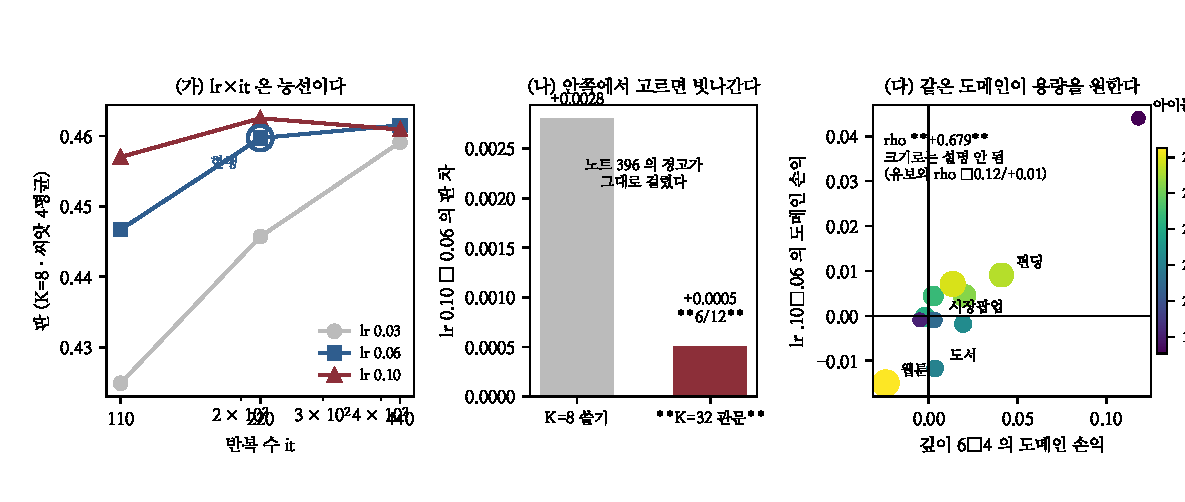
\includegraphics[width=\textwidth]{figs/fig408.pdf}
\caption{(가) lr$\times$it 능선. (나) $K{=}8$ 에서 고른 점이 $K{=}32$ 에서
$+0.0028 \to +0.0005$ 로 녹는다. (다) 두 용량 손잡이의 도메인별 손익
($\rho = +0.679$). 점 크기·색이 유보 행 수인데 크기로는 안 갈린다.}
\end{figure}

\end{document}
